\documentclass[12pt]{article}
\usepackage{tikz}

\begin{document}

\begin{center}
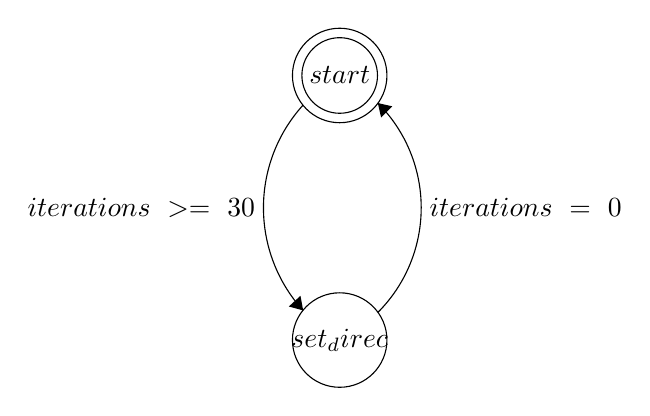
\begin{tikzpicture}[scale=0.2]
\tikzstyle{every node}+=[inner sep=0pt]
\draw [black] (34.8,-17.6) circle (3);
\draw (34.8,-17.6) node {$start$};
\draw [black] (34.8,-17.6) circle (2.4);
\draw [black] (34.8,-34.4) circle (3);
\draw (34.8,-34.4) node {$set_direc$};
\draw [black] (32.476,-32.522) arc (-137.78796:-222.21204:9.707);
\fill [black] (32.48,-32.52) -- (32.31,-31.59) -- (31.57,-32.27);
\draw (29.46,-26) node [left] {$iterations\mbox{ }>=\mbox{ }30$};
\draw [black] (37.221,-19.35) arc (45.01132:-45.01132:9.403);
\fill [black] (37.22,-19.35) -- (37.43,-20.27) -- (38.14,-19.56);
\draw (40.48,-26) node [right] {$iterations\mbox{ }=\mbox{ }0$};
\end{tikzpicture}
\end{center}

\end{document}
